\documentclass[Main]{subfiles}
\begin{document}

\chapter{Indledning}

\section{Formål}

\section{Valg af trådløs kommunikation}

Der er flere krav til den trådløse sender;

\begin{itemize}
\item Regler
\item Frekvens
\item Data bus
\item Hastighed
\end{itemize}

\subsection{Regler og valg af Frekvens}
Der er mange regler inden for trådløs kommunikation, så hvilke frekvenser er lovlige at udnytte uden licens?

Det er de fleste i ISM-båndet, da de er lavet til  Industriel, videnskabelig og medicinsk bånd. Grunden til det ikke er alle er at der er lokale krav, alt efter hvor man er i verden. Eks har USA meget komplekse krav til 433MHZ.\cite[s. 32]{Lov1}

De meste gængse frekvenser der er kan benyttes i industrien og til hobby brug er derfor:

\begin{itemize}
\item 433 MHz
\item 868 MHz
\item 915 MHz
\item 2.4 GHz
\item 5.8 GHz
\end{itemize}

Så der skal vælges en frekvens af disse.
Den frekvens der egner sig bedst dette projekt, er den frekvens der rækker længst. 

\begin{figure}[H]
\centering
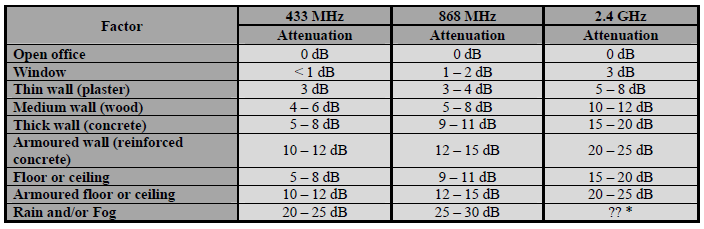
\includegraphics[scale=1]{FrekvensDempning}
\caption{Frekvens dempning - Figuren viser tests udfør af Telit wireless solutions et stort italiensk firma med speciale i trådløs teknologi.}
\end{figure}




Som man det ses på figures over så er der mindre modstand i objekter, desto længere man kommer ned i frekvens.
I og med at næsten alle hobby entusiaster inden for RC fly, bruger 2.4 GHz. 
Bliver valget for dette projekt 433MHz.


\end{document}